\documentclass[12pt,a4paper]{report}

\usepackage{graphicx}
\usepackage{amsmath}
\usepackage{float}
\usepackage{setspace}
\usepackage{geometry}
\usepackage{hyperref}
\usepackage{tikz}
\usetikzlibrary{shapes.geometric, arrows.meta, positioning, calc}
\usepackage{longtable}
\usepackage{array}
\usepackage{booktabs}
\usepackage{enumitem}

\geometry{margin=1in}
\onehalfspacing

\newcolumntype{L}[1]{>{\raggedright\arraybackslash}p{#1}}

\begin{document}

%========================= TITLE PAGE =========================%
\begin{titlepage}
    \centering

    {\small UCS503 -- Software Engineering Lab \hfill}\\[1.5cm]

    {\Large \textbf{UCS 503 Software Engineering Project Report}}\\[0.3cm]
    {\large \textbf{Mid-Semester Evaluation}}\\[1.5cm]

    {\fontsize{18}{24}\selectfont \bfseries Autonomous Agentic Digital Twin for Predictive Maintenance and Closed-Loop Control of Turbofan Engines\par}
    \vspace{1.5cm}

    {\large \textbf{Submitted by}}\\[0.9cm]
    (1024030390) Aakriti\\
    (1024030391) Shruti\\
    (1024030465) Jaivesh\\
    (1024030267) Anoushka\\[1cm]

    \textbf{BE Third Year, CoE}\\
    \textbf{Group No:} 3C25\\[0.5cm]

    \textbf{Submitted to}\\
    Dr. Stuti\\[1.5cm]

    \vfill

    \textbf{Computer Science and Engineering Department}\\
    \textbf{TIET, Patiala}

\end{titlepage}

%========================= TOC =========================%
\tableofcontents
\newpage

%========================================================%
\chapter{Project Selection Phase}
\section{Software Bid}
 
\subsection*{Project Title}
Autonomous Agentic Digital Twin for Predictive Maintenance and Closed-Loop Control of Turbofan Engines
 
\subsection*{Team Details}
\begin{table}[h]
\centering
\begin{tabular}{|c|c|c|c|}
\hline
\textbf{S.No.} & \textbf{Roll Number} & \textbf{Name} & \textbf{Branch / Year} \\
\hline
1 & 1024030390 & Aakriti  & BE CoE, 3rd Year \\
\hline
2 & 1024030391 & Shruti   & BE CoE, 3rd Year \\
\hline
3 & 1024030465 & Jaivesh  & BE CoE, 3rd Year \\
\hline
4 & 1024030267 & Anoushka & BE CoE, 3rd Year \\
\hline
\end{tabular}
\end{table}
 
\subsection*{Problem Domain}
Prognostics and Health Management (PHM) --- Deep Learning-based Remaining Useful Life (RUL) Prediction using the NASA C-MAPSS benchmark dataset, combined with a rule-based policy simulation and Human-in-the-Loop (HITL) approval governance for maintenance decision-making.

\subsection*{Why this Project}
Standard predictive maintenance research typically stops at prediction -- a model estimates Remaining Useful Life (RUL) and leaves the interpretation and decision-making entirely to a human engineer. This project goes one step further: instead of just outputting a number, the system also decides and explains what action should follow from that number, and simulates the effect of that action on the engine's future health.
 
Using the NASA C-MAPSS benchmark dataset, we train an LSTM model to predict RUL from historical sensor readings. On top of this prediction, a rule-based policy layer checks the RUL against defined risk thresholds (Caution, Warning, Critical) and recommends an appropriate action -- such as a graded thrust derate -- along with a clear, logged reason for that choice (e.g., `RUL predicted at 32 cycles, below Warning threshold of 35; derate recommended to extend time-on-wing''). The recommendation, and the reasoning behind it, is presented to the Maintenance Engineer on the dashboard; the action is applied to the digital twin only after the engineer approves it, at which point the simulation updates and shows the resulting change in the engine's wear-rate trajectory. This keeps a human in the loop for every control decision while still automating the analysis, the decision logic, and the justification behind it.
 
This turns a passive prediction system into a prescriptive one: the value isn't just knowing when an engine might fail, but automatically recommending -- and justifying -- what to do about it before it does, while leaving the final call to the engineer. The entire system is built and evaluated offline using the public C-MAPSS dataset, demonstrating the full software engineering lifecycle from data preprocessing and model training to decision logic and dashboard visualization.

\subsection*{Objectives}
\begin{itemize}
    \item Train a PyTorch LSTM model to predict Remaining Useful Life (RUL) from multivariate turbofan sensor telemetry.
    \item Design a policy agent that maps predicted RUL to graded thrust-derate action recommendations using defined risk thresholds.
    \item Provide a human-in-the-loop approval mechanism, allowing the Maintenance Engineer to accept or reject a recommended action before it is applied to the digital twin.
    \item Build a closed-loop simulation showing measurable time-on-wing extension when a recommended action is approved and applied, versus a passive baseline where it is not.
    \item Generate an auditable, human-readable rationale for every recommended control action, to support the engineer's decision.
    \item Deliver an interactive Streamlit dashboard for real-time monitoring, action approval, and ERP work-order dispatch.
\end{itemize}
 
\subsection*{Feasibility Summary}
\begin{itemize}
    \item \textbf{Technical Feasibility:} NASA C-MAPSS dataset , PyTorch deep learning framework, Streamlit interactive web dashboard, and Python-based policy simulation engines.
    \item \textbf{Economic Feasibility:} Entirely open-source software stack (PyTorch, Pandas, NumPy, Streamlit); no proprietary hardware or paid licensing required.
    \item \textbf{Data Feasibility:} NASA C-MAPSS is a publicly available, pre-labeled run-to-failure dataset, eliminating data-collection or sensor procurement risk during the project timeline.
    \item \textbf{Time Feasibility:} Scope is structured into four decoupled software modules (Data/Twin, Prognostics, Policy Agent, Dashboard/API), allowing parallel development across a 4-member team within the semester deadline.
\end{itemize}
 
\subsection*{Risks}
\begin{itemize}
    \item Model accuracy (RMSE) may vary across the four C-MAPSS sub-datasets (FD001--FD004) due to differing operating conditions and fault modes.
    \item Fixed-threshold policy logic may not generalize well if engine degradation patterns deviate from those seen in training data.
    \item Simulated wear-rate reduction under derating is a modeling assumption, not physically validated hardware data.
    \item Since the engineer must approve a recommended action before it is applied, delayed or absent approval will leave the digital twin on the passive degradation trajectory -- this is expected behaviour, not a system fault, but should be clearly communicated during evaluation.
\end{itemize}

\section{Project Overview}
 
\subsection*{Overview}
This project builds a Digital Twin framework that mirrors a physical turbofan engine using its sensor and operational-cycle data. A deep learning model (LSTM-based) is trained on the NASA C-MAPSS dataset to learn degradation patterns and predict the Remaining Useful Life of an engine. The predicted RUL is then used to classify the engine's health condition and support predictive maintenance decisions.
 
\subsection*{Scope}
\begin{itemize}
    \item Preprocessing and labeling of the C-MAPSS \textbf{FD001} sub-dataset, used for model training, the policy agent, and the dashboard demo in this evaluation.
    \item Training a sequence model (LSTM) for RUL regression.
    \item A Digital Twin view that reflects predicted engine health in near real time from historical/simulated sensor streams.
    \item Evaluation using MAE, RMSE and R\textsuperscript{2}.
\end{itemize}
 
\subsection*{Out of Scope}
\begin{itemize}
    \item C-MAPSS sub-datasets FD002, FD003, and FD004 -- deferred to a stretch goal if time permits.
    \item Integration with physical/live IoT sensors on a real engine.
    \item Certification-grade safety validation.
\end{itemize}
 
\subsection*{Stakeholders}
\begin{itemize}
    \item Maintenance Engineer (primary user of RUL predictions).
    \item Fleet/Operations Manager (maintenance scheduling decisions).
    \item Data Science Team (model training and monitoring).
\end{itemize}

\section{Software Development Life Cycle (SDLC) Model}

For this project, an \textbf{Iterative \& Agile Scrum SDLC Model} was selected due to the experimental nature of deep learning model training coupled with rigorous software engineering and cyber-physical control requirements.

\begin{figure}[H]
\centering
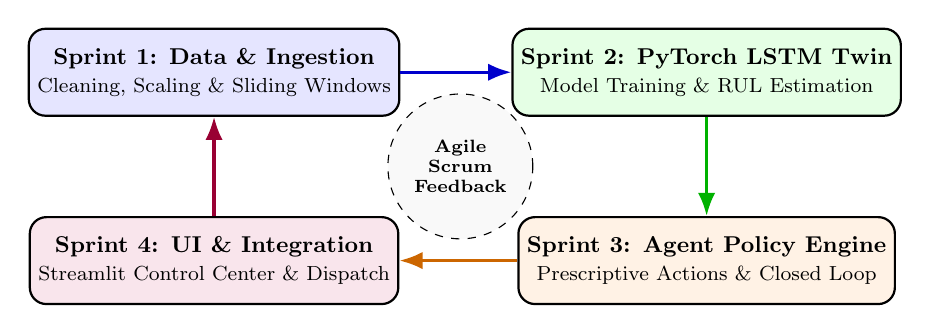
\begin{tikzpicture}[
    scale=0.92, transform shape,
    every node/.style={font=\small},
    sprint/.style={draw, rounded corners=6pt, align=center, minimum width=4.8cm, minimum height=1.2cm, thick}
]
    \node[sprint, fill=blue!10] (s1) at (0, 2.6) {\textbf{Sprint 1: Data \& Ingestion}\\ \footnotesize Cleaning, Scaling \& Sliding Windows};
    \node[sprint, fill=green!10] (s2) at (6.8, 2.6) {\textbf{Sprint 2: PyTorch LSTM Twin}\\ \footnotesize Model Training \& RUL Estimation};
    \node[sprint, fill=orange!10] (s3) at (6.8, 0) {\textbf{Sprint 3: Agent Policy Engine}\\ \footnotesize Prescriptive Actions \& Closed Loop};
    \node[sprint, fill=purple!10] (s4) at (0, 0) {\textbf{Sprint 4: UI \& Integration}\\ \footnotesize Streamlit Control Center \& Dispatch};

    \draw[-Latex, very thick, blue!80!black] (s1.east) -- (s2.west);
    \draw[-Latex, very thick, green!70!black] (s2.south) -- (s3.north);
    \draw[-Latex, very thick, orange!80!black] (s3.west) -- (s4.east);
    \draw[-Latex, very thick, purple!80!black] (s4.north) -- (s1.south);

    \node[draw, dashed, circle, fill=gray!5, minimum size=2.0cm, align=center, font=\scriptsize] at (3.4, 1.3) {\textbf{Agile}\\ \textbf{Scrum}\\ \textbf{Feedback}};
\end{tikzpicture}
\caption{Iterative Agile SDLC Workflow for Cyber-Physical Digital Twin}
\label{fig:sdlc}
\end{figure}

\begin{itemize}[leftmargin=0.6cm]
    \item \textbf{Sprint 1 (Weeks 1--3):} Data curation, exploratory data analysis of C-MAPSS FD001--FD004, constant sensor filtering, and sliding window sequence generation.
    \item \textbf{Sprint 2 (Weeks 4--6):} PyTorch LSTM architecture development, hyperparameter tuning, training pipeline, and validation against NASA benchmark metrics.
    \item \textbf{Sprint 3 (Weeks 7--9):} Development of the autonomous policy agent, risk-cost evaluation matrices, and closed-loop wear-reduction simulation.
    \item \textbf{Sprint 4 (Weeks 10--12):} Streamlit interactive dashboard, physical parameter injection sliders, Human-in-the-Loop review and approval interface, and JSON work-order generator.
\end{itemize}
 
%========================================================%
\chapter{Analysis Phase}
\section{Use Cases}
The system has one primary actor, the \textbf{Maintenance Engineer}, and one supporting actor, the \textbf{Digital Twin System} itself (automated actor that periodically ingests sensor data, triggers predictions, and generates maintenance action recommendations). The Digital Twin System proposes an action when the predicted RUL crosses a defined risk threshold, but the Maintenance Engineer retains final control -- reviewing the recommendation and its rationale before deciding whether it is applied to the digital twin.

\subsection{Use-Case Diagrams}
\label{sec:usecasediagram}

\begin{figure}[H]
\centering
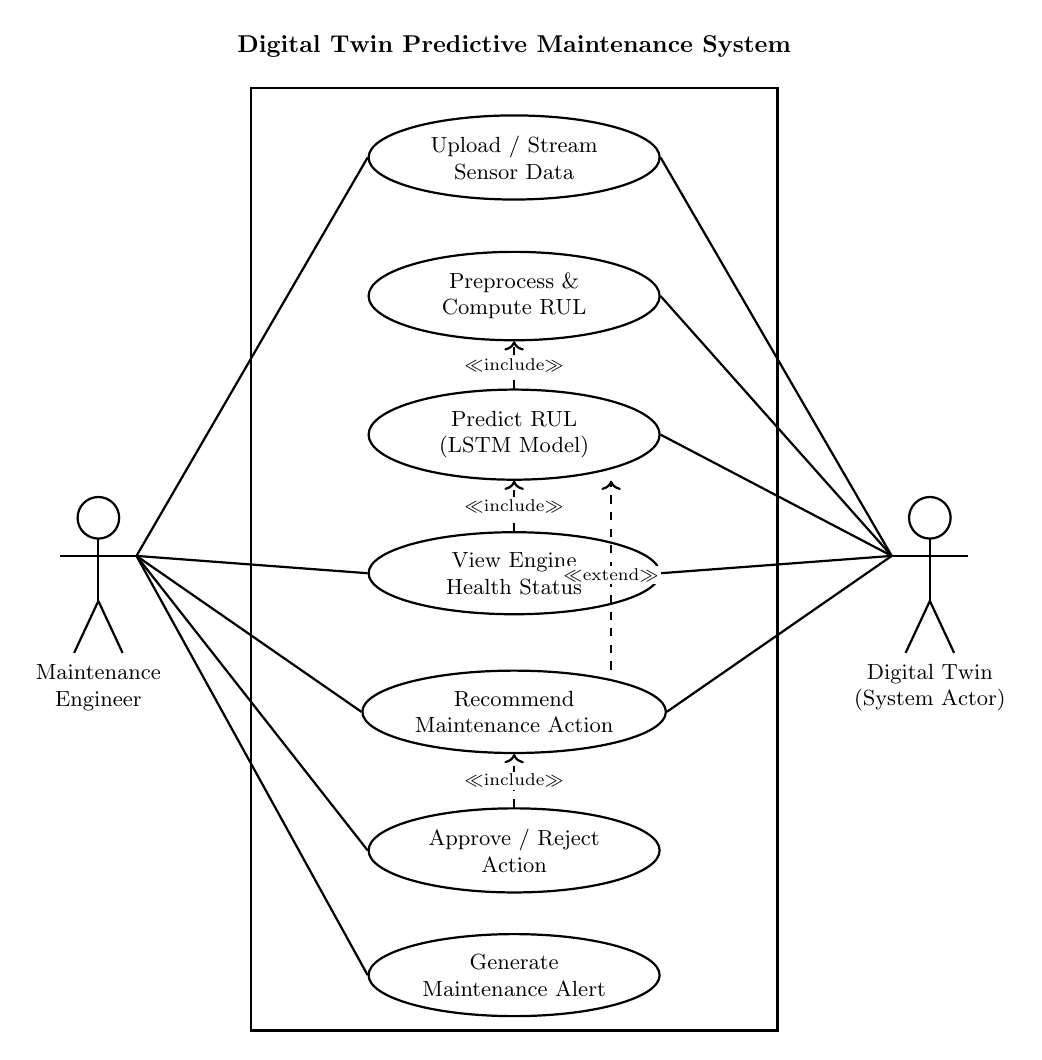
\begin{tikzpicture}[
    scale=0.88, transform shape,
    every node/.style={align=center},
    usecase/.style={draw, ellipse, minimum width=4.2cm, minimum height=0.9cm, font=\small, fill=white, thick}
]

    % Title ABOVE the box
    \node[font=\bfseries] at (0, 8.2) {Digital Twin Predictive Maintenance System};

    % System boundary rectangle (title sits outside, above)
    \draw[thick] (-3.8, -6.0) rectangle (3.8, 7.6);

    % Use-case ellipses — evenly spaced vertically
    \node[usecase] (uc1) at (0, 6.6) {Upload / Stream\\Sensor Data};
    \node[usecase] (uc2) at (0, 4.6) {Preprocess \&\\Compute RUL};
    \node[usecase] (uc3) at (0, 2.6) {Predict RUL\\(LSTM Model)};
    \node[usecase] (uc4) at (0, 0.6) {View Engine\\Health Status};
    \node[usecase] (uc5) at (0, -1.4) {Recommend\\Maintenance Action};
    \node[usecase] (uc6) at (0, -3.4) {Approve / Reject\\Action};
    \node[usecase] (uc7) at (0, -5.2) {Generate\\Maintenance Alert};

    % Left Actor: Maintenance Engineer
    \node (eng_head) at (-6.0, 1.4) {};
    \draw[thick] (eng_head) circle (0.3);
    \draw[thick] (-6.0, 1.1) -- (-6.0, 0.2);
    \draw[thick] (-6.55, 0.85) -- (-5.45, 0.85);
    \draw[thick] (-6.0, 0.2) -- (-6.35, -0.55);
    \draw[thick] (-6.0, 0.2) -- (-5.65, -0.55);
    \node[font=\small] at (-6.0, -1.05) {Maintenance\\Engineer};
    \coordinate (eng_hand) at (-5.45, 0.85);

    % Right Actor: Digital Twin (System Actor)
    \node (twin_head) at (6.0, 1.4) {};
    \draw[thick] (twin_head) circle (0.3);
    \draw[thick] (6.0, 1.1) -- (6.0, 0.2);
    \draw[thick] (5.45, 0.85) -- (6.55, 0.85);
    \draw[thick] (6.0, 0.2) -- (5.65, -0.55);
    \draw[thick] (6.0, 0.2) -- (6.35, -0.55);
    \node[font=\small] at (6.0, -1.05) {Digital Twin\\(System Actor)};
    \coordinate (twin_hand) at (5.45, 0.85);

    % Left connections (Maintenance Engineer)
    \draw[thick] (eng_hand) -- (uc1.west);
    \draw[thick] (eng_hand) -- (uc4.west);
    \draw[thick] (eng_hand) -- (uc5.west);
    \draw[thick] (eng_hand) -- (uc6.west);
    \draw[thick] (eng_hand) -- (uc7.west);

    % Right connections (Digital Twin System Actor)
    \draw[thick] (twin_hand) -- (uc1.east);
    \draw[thick] (twin_hand) -- (uc2.east);
    \draw[thick] (twin_hand) -- (uc3.east);
    \draw[thick] (twin_hand) -- (uc4.east);
    \draw[thick] (twin_hand) -- (uc5.east);

    % Include arrows (straight vertical dashed, pointing UP)
    \draw[dashed, ->, thick] (uc3.north) -- node[midway, fill=white, inner sep=1pt, font=\scriptsize] {$\ll$include$\gg$} (uc2.south);
    \draw[dashed, ->, thick] (uc4.north) -- node[midway, fill=white, inner sep=1pt, font=\scriptsize] {$\ll$include$\gg$} (uc3.south);
    \draw[dashed, ->, thick] (uc6.north) -- node[midway, fill=white, inner sep=1pt, font=\scriptsize] {$\ll$include$\gg$} (uc5.south);

    % Extend arrow — slightly offset right, straight vertical from uc5 up to uc3 (bypassing uc4)
    \draw[dashed, ->, thick] ([xshift=1.4cm]uc5.north) -- node[pos=0.5, fill=white, inner sep=1pt, font=\scriptsize] {$\ll$extend$\gg$} ([xshift=1.4cm]uc3.south);

\end{tikzpicture}
\caption{Use-Case Diagram for the Digital Twin Predictive Maintenance System}
\label{fig:usecase}
\end{figure}

\subsection{Use Case Templates}

\begin{longtable}{L{3.2cm} L{9.5cm}}
\toprule
\multicolumn{2}{l}{\textbf{Use Case: Predict RUL (LSTM Model)}} \\
\midrule
Use Case ID & UC-03 \\
Actor(s) & Digital Twin System \\
Description & The system processes a sequence of turbofan engine sensor readings and uses the trained LSTM model to predict the Remaining Useful Life (RUL) of the engine. \\
Preconditions & Sensor data is available and preprocessed; required features have been normalized/scaled; a trained LSTM model is available. \\
Main Flow &
1. System receives the latest sequence of engine sensor readings.\\
& 2. System preprocesses and prepares the sensor sequence for inference.\\
& 3. System feeds the sequence into the trained LSTM model.\\
& 4. LSTM model generates the predicted RUL value.\\
& 5. System forwards the predicted RUL to the health-status and policy modules.\\
Postconditions & A predicted RUL value is generated and available for health assessment and maintenance decision-making. \\
\bottomrule
\end{longtable}

\begin{longtable}{L{3.2cm} L{9.5cm}}
\toprule
\multicolumn{2}{l}{\textbf{Use Case: Generate Maintenance Recommendation}} \\
\midrule
Use Case ID & UC-04 \\
Actor(s) & Digital Twin System, Maintenance Engineer \\
Description & The system evaluates the predicted RUL against predefined risk thresholds and generates an appropriate maintenance or control action recommendation. The recommendation is presented to the Maintenance Engineer for approval before being applied to the Digital Twin. \\
Preconditions & A valid RUL prediction has been generated; risk thresholds and corresponding maintenance policies are configured. \\
Main Flow &
1. System receives the predicted RUL from the RUL prediction module.\\
& 2. System compares the predicted RUL with the defined health/risk thresholds.\\
& 3. System determines the appropriate action based on the engine's health condition.\\
& 4. System generates a maintenance recommendation along with a human-readable rationale.\\
& 5. System displays the predicted RUL, health status, recommended action, and rationale on the dashboard.\\
& 6. Maintenance Engineer reviews the recommendation.\\
& 7. Engineer approves the recommended action.\\
& 8. System applies the approved action to the Digital Twin simulation.\\
& 9. Digital Twin updates the engine's simulated degradation/wear-rate trajectory based on the applied action.\\
& 10. System displays the updated engine health and estimated time-on-wing extension.\\
Postconditions & The approved action is applied to the Digital Twin and the resulting change in the engine's degradation trajectory is recorded and displayed. \\
\bottomrule
\end{longtable}

\section{Activity Diagram and Swimlane Diagrams}

\begin{figure}[H]
\centering
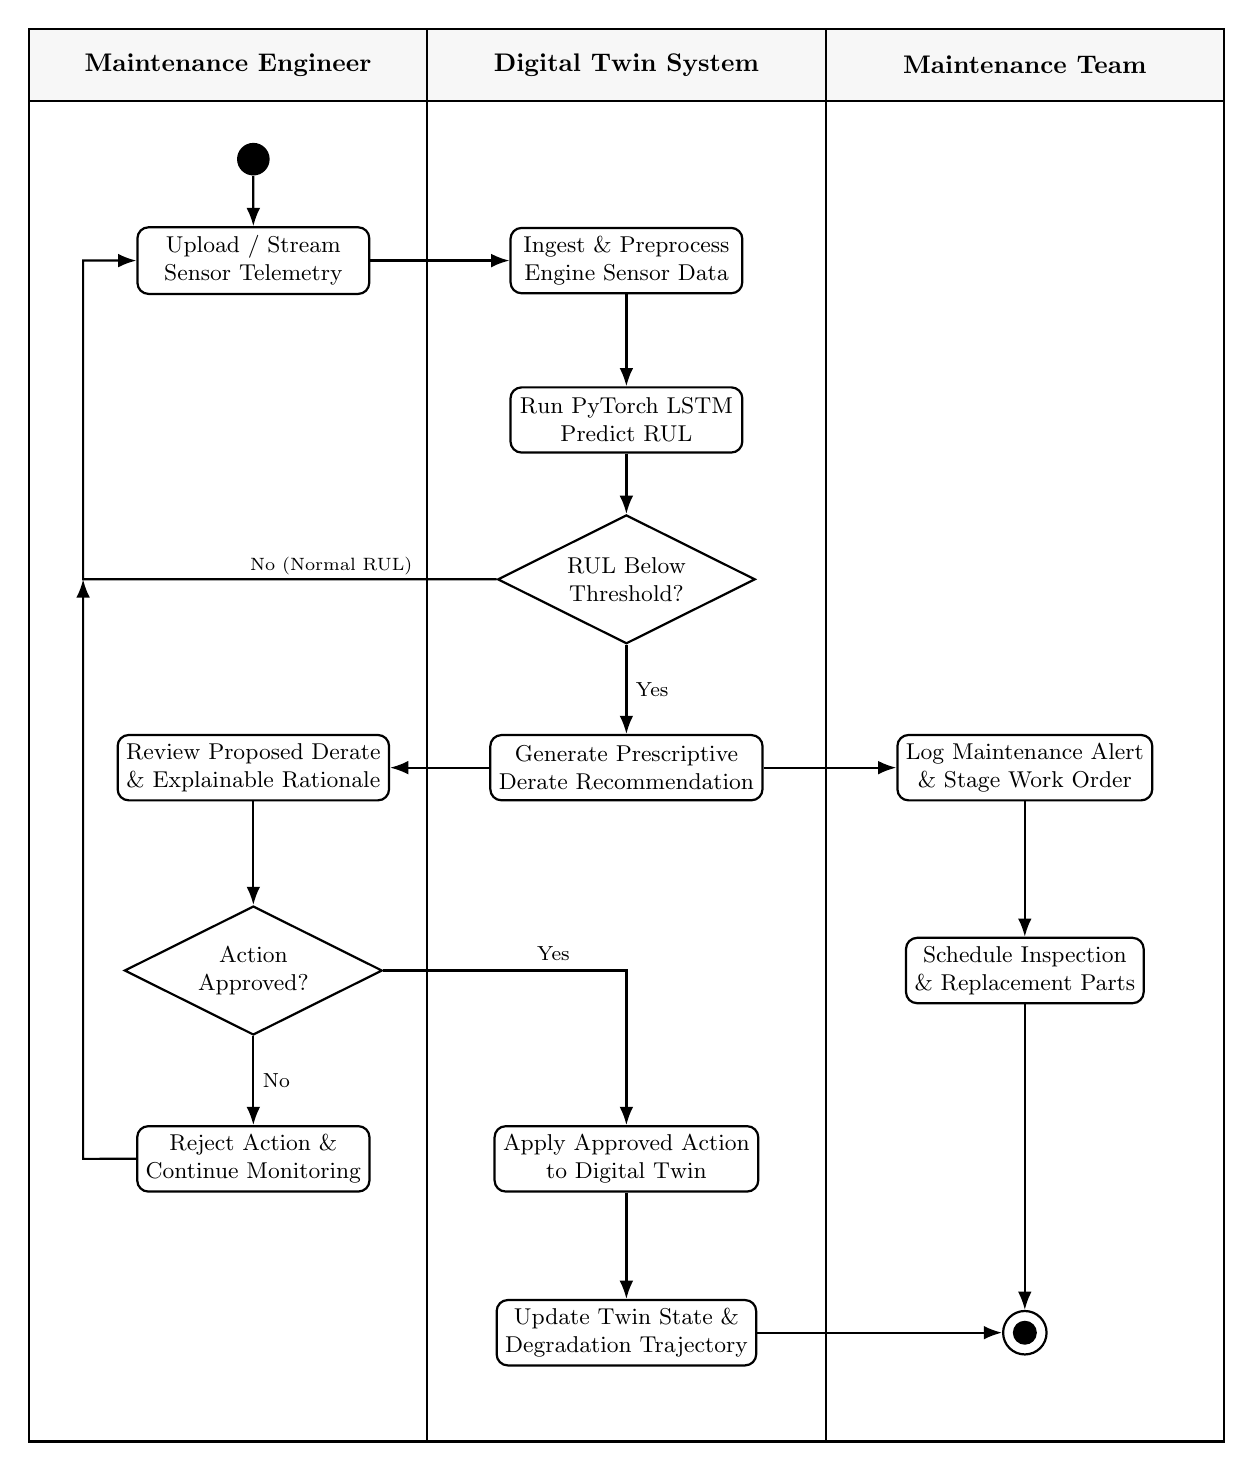
\begin{tikzpicture}[
    scale=0.92, transform shape,
    font=\small,
    >=Latex,
    act/.style={
        draw, rounded corners=4pt, minimum width=3.2cm, minimum height=0.9cm, align=center, fill=white, thick
    },
    dec/.style={
        draw, diamond, aspect=2.0, minimum width=2.8cm, minimum height=1.0cm, align=center, fill=white, thick
    },
    flow/.style={->, thick}
]

% SWIMLANES (Total width 16.5cm, height 19.5cm)
\fill[gray!6] (0,0) rectangle (16.5,-1.0);
\draw[thick] (0,0) rectangle (5.5,-19.5);
\node[font=\normalsize\bfseries] at (2.75,-0.5) {Maintenance Engineer};

\draw[thick] (5.5,0) rectangle (11.0,-19.5);
\node[font=\normalsize\bfseries] at (8.25,-0.5) {Digital Twin System};

\draw[thick] (11.0,0) rectangle (16.5,-19.5);
\node[font=\normalsize\bfseries] at (13.75,-0.5) {Maintenance Team};

\draw[thick] (0,-1.0) -- (16.5,-1.0);

% START NODE
\node[circle, fill=black, minimum size=0.45cm] (start) at (3.1,-1.8) {};

% ACTIVITIES
\node[act] (upload) at (3.1,-3.2) {Upload / Stream\\Sensor Telemetry};
\node[act] (preprocess) at (8.25,-3.2) {Ingest \& Preprocess\\Engine Sensor Data};
\node[act] (predict) at (8.25,-5.4) {Run PyTorch LSTM\\Predict RUL};
\node[dec] (threshold) at (8.25,-7.6) {RUL Below\\Threshold?};

\node[act] (generate) at (8.25,-10.2) {Generate Prescriptive\\Derate Recommendation};
\node[act] (review) at (3.1,-10.2) {Review Proposed Derate\\\& Explainable Rationale};
\node[act] (alert) at (13.75,-10.2) {Log Maintenance Alert\\\& Stage Work Order};

\node[dec] (approve) at (3.1,-13.0) {Action\\Approved?};
\node[act] (schedule) at (13.75,-13.0) {Schedule Inspection\\\& Replacement Parts};

\node[act] (reject) at (3.1,-15.6) {Reject Action \&\\Continue Monitoring};
\node[act] (apply) at (8.25,-15.6) {Apply Approved Action\\to Digital Twin};

\node[act] (update) at (8.25,-18.0) {Update Twin State \&\\Degradation Trajectory};

% END NODE
\node[circle, draw, thick, minimum size=0.6cm] (endouter) at (13.75,-18.0) {};
\node[circle, fill=black, minimum size=0.3cm] at (13.75,-18.0) {};

% FLOWS
\draw[flow] (start) -- (upload);
\draw[flow] (upload.east) -- (preprocess.west);
\draw[flow] (preprocess.south) -- (predict.north);
\draw[flow] (predict.south) -- (threshold.north);

% Loop back from threshold (No)
\draw[flow] (threshold.west) -- node[pos=0.4, above, font=\scriptsize, fill=white, inner sep=1.5pt] {No (Normal RUL)} (0.75,-7.6) -- (0.75,-3.2) -- (upload.west);

% Yes: down to Generate
\draw[flow] (threshold.south) -- node[right, font=\footnotesize]{Yes} (generate.north);

% Generate to Review and Alert
\draw[flow] (generate.west) -- (review.east);
\draw[flow] (generate.east) -- (alert.west);
\draw[flow] (alert.south) -- (schedule.north);

% Review to Approve
\draw[flow] (review.south) -- (approve.north);

% Approve: No -> Reject
\draw[flow] (approve.south) -- node[right, font=\footnotesize]{No} (reject.north);

% Approve: Yes -> Apply
\draw[flow] (approve.east) -| node[pos=0.35, above, font=\footnotesize]{Yes} (apply.north);

% Apply -> Update
\draw[flow] (apply.south) -- (update.north);

% Update -> End
\draw[flow] (update.east) -- (endouter.west);

% Schedule -> End
\draw[flow] (schedule.south) -- (endouter.north);

% Reject: Loop back
\draw[flow] (reject.west) -- (0.75,-15.6) -- (0.75,-7.6);

\end{tikzpicture}
\caption{Activity / Swimlane Diagram for Closed-Loop Predictive Maintenance}
\label{fig:activity}
\end{figure}

\section{Class Diagram and Sequence Diagram}

\subsection{Class Diagram}
The class diagram captures the static structural design of the Digital Twin system, detailing the core entity classes, controller services, their attributes, methods, and relationships.

\begin{figure}[H]
\centering
\includegraphics[width=\textwidth]{class_diagram.png}
\caption{Class Diagram for the Digital Twin Predictive Maintenance System}
\label{fig:class_diagram}
\end{figure}

\subsection{Sequence Diagram}
The sequence diagram models the dynamic runtime interactions and message-flow sequences across the Maintenance Engineer, System Gateway, LSTM Inference Engine, and Digital Twin Simulation Engine during the predictive maintenance lifecycle.

\begin{figure}[H]
\centering
\includegraphics[width=\textwidth]{sequence_diagram.png}
\caption{Sequence Diagram for Closed-Loop Predictive Maintenance Workflow}
\label{fig:sequence_diagram}
\end{figure}

% =========================================================
% DATA FLOW DIAGRAMS
% =========================================================

\section{Data Flow Diagrams}

\subsection{DFD Level 0 (Context Diagram)}

\begin{figure}[H]
\centering
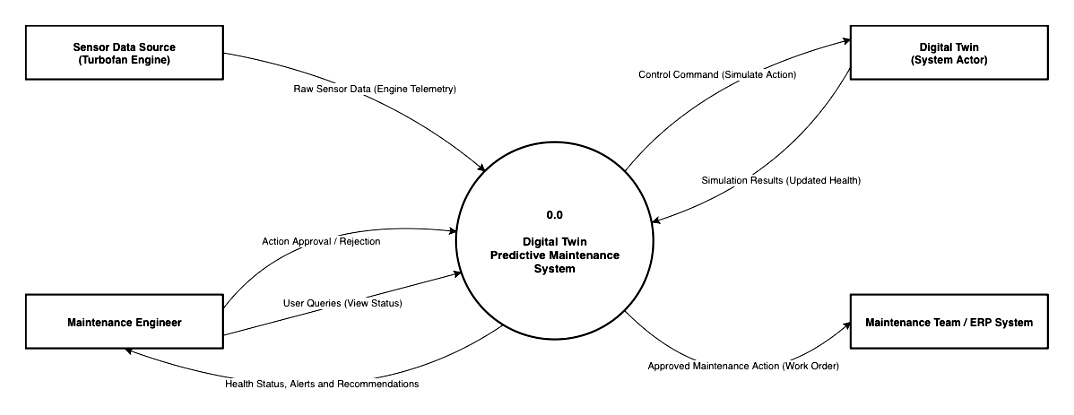
\includegraphics[width=\textwidth]{dfd0.png}
\caption{DFD Level 0 (Context Diagram) for the Digital Twin Predictive Maintenance System}
\label{fig:dfd0}
\end{figure}

\subsection{DFD Level 1}

\begin{figure}[H]
\centering
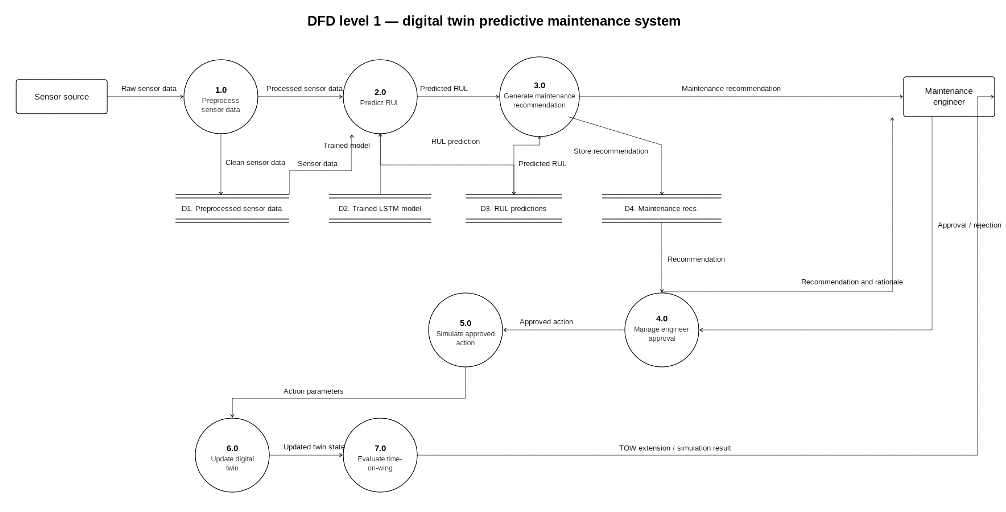
\includegraphics[width=\textwidth]{dfd1.png}
\caption{DFD Level 1 for the Digital Twin Predictive Maintenance System}
\label{fig:dfd1}
\end{figure}

\subsection{DFD Level 2 (Decomposition of Process 2.0 -- Predict RUL)}

\begin{figure}[H]
\centering
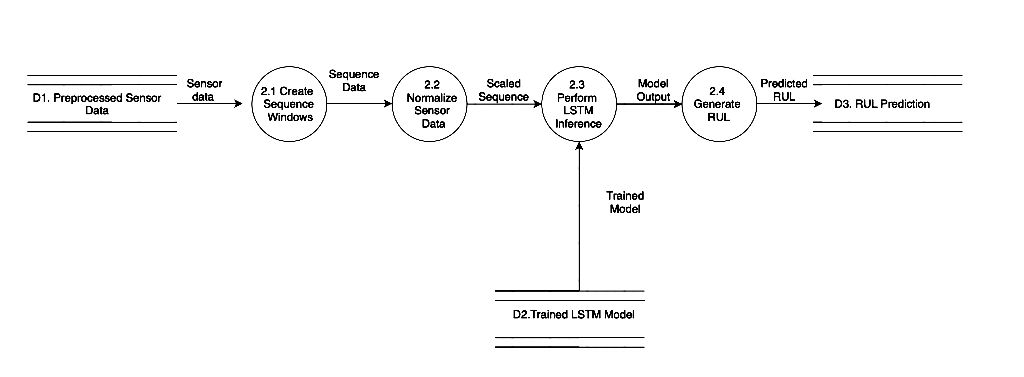
\includegraphics[width=\textwidth]{dfd2.png}
\caption{DFD Level 2 -- Decomposition of Process 2.0 (Predict RUL)}
\label{fig:dfd2}
\end{figure}

\section{Software Requirement Specification in IEEE Format}

\subsection*{1. Introduction}

\subsubsection*{1.1 Purpose}
This document specifies the software requirements for the Autonomous Agentic Digital Twin for Predictive Maintenance and Closed-Loop Control of Turbofan Engines. The system uses historical turbofan engine sensor data to predict Remaining Useful Life (RUL) using an LSTM-based deep learning model. Based on the predicted RUL, the system provides maintenance recommendations and supports the Maintenance Engineer in making informed maintenance decisions.

\subsubsection*{1.2 Scope}
The system covers the complete software workflow for predictive maintenance of turbofan engines, including sensor data preprocessing, LSTM-based RUL prediction, engine health assessment, maintenance action recommendation, and human-in-the-loop approval. An approved action is applied to the Digital Twin simulation to update the engine's degradation trajectory and evaluate its effect on the engine's remaining operating life.

The system is developed and evaluated offline using the NASA C-MAPSS FD001--FD004 datasets. Integration with physical turbofan engines, live IoT sensors, and certification-grade safety validation is outside the scope of this project.

\subsubsection*{1.3 Definitions, Acronyms and Abbreviations}
\begin{itemize}
    \item \textbf{RUL} -- Remaining Useful Life
    \item \textbf{LSTM} -- Long Short-Term Memory
    \item \textbf{C-MAPSS} -- Commercial Modular Aero-Propulsion System Simulation
    \item \textbf{PHM} -- Prognostics and Health Management
    \item \textbf{Digital Twin} -- A virtual representation of a turbofan engine used to monitor its health and simulate its degradation.
    \item \textbf{TOW} -- Time-on-Wing
    \item \textbf{HITL} -- Human-in-the-Loop
\end{itemize}

\subsection*{2. Overall Description}

\subsubsection*{2.1 Product Perspective}
The system is a standalone predictive maintenance application that combines an LSTM-based RUL predictor with a Digital Twin and rule-based maintenance recommendation module.

\subsubsection*{2.2 Product Functions}
\begin{itemize}
    \item Ingest and preprocess turbofan sensor data.
    \item Predict RUL using the trained LSTM model.
    \item Assess engine health and generate maintenance recommendations.
    \item Obtain engineer approval and simulate the approved action.
    \item Display engine health, predictions, and simulation results.
\end{itemize}

\subsubsection*{2.3 User Classes and Characteristics}
\textbf{Maintenance Engineer:} Reviews engine health, RUL predictions, and maintenance recommendations, and approves or rejects proposed actions.

\subsubsection*{2.4 Operating Environment}
Python-based application using PyTorch, Pandas, and NumPy, with a Streamlit-based dashboard for system interaction and visualization.

\subsection*{3. Specific Requirements}

\subsubsection*{3.1 Functional Requirements}
\begin{itemize}
    \item \textbf{FR-1:} The system shall accept turbofan engine sensor data in CSV format compatible with the NASA C-MAPSS dataset.
    \item \textbf{FR-2:} The system shall preprocess sensor data and generate RUL labels for training using $\text{RUL}_i = \text{Maximum Cycle} - \text{Current Cycle}$.
    \item \textbf{FR-3:} The system shall predict RUL for a given engine sequence using the trained LSTM model.
    \item \textbf{FR-4:} The system shall classify the predicted RUL into predefined health conditions.
    \item \textbf{FR-5:} The system shall generate a maintenance recommendation based on the predicted RUL and defined risk thresholds.
    \item \textbf{FR-6:} The system shall display the predicted RUL, health status, recommended action, and rationale on the dashboard.
    \item \textbf{FR-7:} The system shall allow the Maintenance Engineer to approve or reject a recommended action.
    \item \textbf{FR-8:} The system shall apply an approved action to the Digital Twin and update the simulated engine degradation trajectory.
    \item \textbf{FR-9:} The system shall compare the intervention and passive degradation trajectories to estimate time-on-wing extension.
\end{itemize}

\subsubsection*{3.2 Non-Functional Requirements}
\begin{itemize}
    \item \textbf{NFR-1 (Performance):} RUL prediction for a single engine shall complete within 2 seconds.
    \item \textbf{NFR-2 (Usability):} The dashboard shall present engine health, RUL, alerts, and recommendations clearly.
    \item \textbf{NFR-3 (Reliability):} Model performance shall be evaluated using MAE, RMSE, and R\textsuperscript{2}.
    \item \textbf{NFR-4 (Maintainability):} Data preprocessing, model prediction, policy logic, and simulation components shall be modular for independent updates and retraining.
\end{itemize}

\subsubsection*{3.3 External Interface Requirements}
\begin{itemize}
    \item \textbf{Input:} NASA C-MAPSS turbofan engine sensor data in CSV format.
    \item \textbf{Output:} RUL predictions, engine health status, maintenance recommendations, alerts, and Digital Twin simulation results.
    \item \textbf{User Interface:} Streamlit-based dashboard for engine monitoring, recommendation review, and action approval.
\end{itemize}

\newpage

\section{User Stories and Story Cards}

\begin{longtable}{L{2.5cm} L{4.5cm} L{2cm} L{2.7cm}}
\toprule
\textbf{ID} & \textbf{User Story} & \textbf{Priority} & \textbf{Story Points} \\
\midrule
US-01 & As a Maintenance Engineer, I want to provide engine sensor data so that the system can analyze the engine condition. & High & 3 \\
US-02 & As a Maintenance Engineer, I want to view the predicted RUL and health status of an engine so that I can plan maintenance. & High & 5 \\
US-03 & As a Maintenance Engineer, I want the system to generate a maintenance recommendation when the predicted RUL indicates increased risk so that I can take appropriate action. & High & 5 \\
US-04 & As a Maintenance Engineer, I want to review and approve or reject a recommended action so that maintenance decisions remain under human control. & High & 3 \\
US-05 & As a Maintenance Engineer, I want to see the effect of an approved action on the Digital Twin so that I can evaluate the resulting engine degradation and time-on-wing extension. & High & 5 \\
US-06 & As a Data Science Team member, I want to evaluate the RUL model using MAE, RMSE, and R\textsuperscript{2} so that I can assess prediction performance. & Medium & 3 \\
\bottomrule
\end{longtable}

\subsection*{Sample Story Card -- US-05}

\begin{longtable}{L{3cm} L{9.5cm}}
\toprule
Story & As a Maintenance Engineer, I want to see the effect of an approved action on the Digital Twin so that I can evaluate the resulting engine degradation and time-on-wing extension. \\
Acceptance Criteria &
1. Given a recommended action, the engineer can approve the action.\\
& 2. The approved action is applied to the Digital Twin simulation.\\
& 3. The Digital Twin updates the simulated engine degradation trajectory.\\
& 4. The system compares the intervention trajectory with the passive baseline.\\
& 5. The system displays the estimated time-on-wing extension resulting from the approved action. \\
Priority & High \\
Estimate & 5 Story Points \\
\bottomrule
\end{longtable}

\end{document}
